\chapter{Introduction}

%%%%%%%%%%%%%
% LECTURE 1 %
%%%%%%%%%%%%%

\lecture{1}{04/10/2021}

\section{Qubits}
The \textbf{bit} is the fundamental concept of classical computation and information. Quantum computation and information are built upon an analogous concept: the \textbf{quantum bit}, or \textbf{qubit}. What is a qubit? Quantum mechanically, a qubit is any two-level system. For example, we can use the two different polarizations of a photon, the alignment of a nuclear spin in a
uniform magnetic field, or the two states of an electron orbiting a single atom or molecule (ammonia-based quantum computer\footnote{Ferguson, A., Cain, P., Williams, D., \& Briggs, G. (2002). Ammonia-based quantum computer. Phys. Rev. A, 65, 034303.}). Just as a classical bit has a \textbf{state} - either 0 or 1 - a qubit also has a \textbf{state}. Two possible states for a qubit are the state $|0\rangle$ and $|1\rangle$ (we use \textit{Dirac notation}\footnote{Also known as bra-ket notation, it is a formalism introduced by Paul Dirac to describe one quantum state. The name derives from the fact that the scalar product of two states $\phi$ and $\psi$ is denoted with a bracket $\langle\phi|\psi\rangle$ consisting of two parts: $\langle\phi|$ the \textit{bra} and $|\psi\rangle$ the \textit{ket}.}). The difference between bits and qubits is that a qubit can be in a state other than $|0\rangle$  or $|1\rangle$. It is also possible to form \textit{linear combinations} of states, often called \textit{superpositions}:

\begin{equation*}
    |\psi\rangle=\alpha|0\rangle + \beta|1\rangle
\end{equation*}

The numbers $\alpha$ and $\beta$ are complex numbers. See in another way, the state of a qubit is a vector in a two-dimensional complex vector space. The special states $|0\rangle$ and $|1\rangle$ are know as computational basis states and form an orthonormal basis for this vector space. We can examine a bit to determine whether it is in the state 0 or 1. For example, computers do this all-time when they retrieve the contents of their memory. Instead, quantum mechanics tells us that we can only acquire much more restricted information about the quantum state. When we measure a qubit, we get either 0 with probability $\alpha$ or 1 with probability $\beta$. Naturally, they must satisfy the following condition:

\begin{equation*}
    |\alpha|^2+|\beta|^2=1
\end{equation*}

Like in a QM system, the phase is irrelevant, it's a degree of freedom. For this reason, qubits could store infinite information. However, this conclusion turn out to be misleading, because of the behavior of a qubit when observed. Remind that the measurement of a qubit will give only either 0 or 1. Furthermore, measurement changes the state of a qubit, collapsing it from its superposition of $|0\rangle$ and $|1\rangle$ to the specific state consistent with the measurement result. From a single measurement one obtains only a single bit of information about the state of the qubit, thus resolving the apparent paradox. It turns out that only if infinitely many identically prepared qubits were measured would one be able to determine $\alpha$ and $\beta$ for a qubit in the state $|\psi\rangle$.

\subsection{Summary for general principles on QM}
\begin{itemize}
    \item \textbf{Postulate I}: What is a state? We use Dirac notation to represents a vector in an Hilbert-space (finite dimension) $|\psi\rangle \in \mathcal{H}$, where the states lives. The states is given by a vector also named as \textit{ray} and it should have a unit norm (conservation of probability) $|| |\psi\rangle ||=1$. All phases are irrelevant $|\psi\rangle \approx e^{i\alpha}|\psi\rangle \ \alpha\in\mathbb{R}$, if two states differs from a phase, they have the same physical effect.
\end{itemize}
If we have two states $|\psi_1\rangle$ and $|\psi_2\rangle$, and we consider their linear combination: $|\psi\rangle = \alpha_1|\psi_1\rangle+\alpha_2|\psi_2\rangle$, then $|\psi\rangle$ is also a state in $\mathcal{H}$. But we need to pay attention for $|\psi\rangle$, we need to normalize it for the conservation of probability.

\begin{definition}[\textbf{Scalar product}]
    We define \textbf{scalar product} the following quantity: $\langle\phi|\psi\rangle$ (\textbf{bra-ket} notation), where $\langle\phi|$ is the dual vector of $|\phi\rangle$.
\end{definition}

\noindent Qubit systems work in $\mathcal{H}=\mathbb{C}^2$. Where a vector $\begin{pmatrix}z_1\\z_2\end{pmatrix}$ has $z_1,z_2\in\mathbb{C}$. We can also say that $|0\rangle$ and $|1\rangle$ are an orthogonal bases:

\begin{equation*}
    |0\rangle = \begin{pmatrix}1\\0\end{pmatrix} \ \ \ \ \ |1\rangle = \begin{pmatrix}0\\1\end{pmatrix}
\end{equation*}

\noindent where their scalar products are:

\begin{equation*}
    \langle0|0\rangle=\langle1|1\rangle=1 \ \ \ \ \ \langle0|1\rangle=\langle1|0\rangle=0
\end{equation*}

\noindent So our general state it can be written as:

\begin{equation*}
    \begin{pmatrix}z_1\\z_2\end{pmatrix}=z_1\begin{pmatrix}1\\0\end{pmatrix} + z_2\begin{pmatrix}0\\1\end{pmatrix}=z_1|0\rangle+z_2|1\rangle
\end{equation*}

\noindent The scalar product between $|\phi\rangle=\begin{pmatrix}z_1\\z_2\end{pmatrix}$ and $|\psi\rangle=\begin{pmatrix}w_1\\w_2\end{pmatrix}$ is defined as:

\begin{equation*}
    \langle\psi|\phi\rangle=w_1^*z_1+w_2^*z_2
\end{equation*}

\noindent If we have $|\phi\rangle = \begin{pmatrix}z_1\\z_2\end{pmatrix}$ (ket), we transpose and conjugate $\langle\phi|=(z_1^*, z_2^*)$ (bra). Then we can rewrite the scalar product as:

\begin{equation*}
    \langle\psi|\phi\rangle=(w_1^*, w_2^*)\begin{pmatrix}z_1\\z_2\end{pmatrix}=w_1^*z_1+w_2^*z_2
\end{equation*}

\noindent Summing up, we can write a generic state as:
\begin{equation*}
    \begin{pmatrix}z_1\\z_2\end{pmatrix}=z_1|0\rangle+z_2|1\rangle
\end{equation*}

\noindent with these two constraints:
\begin{itemize}
    \item \textbf{Conservation of probability}: $|z_1|^2+|z_2|^2=1$
    \item \textbf{Phase invariance}: $\begin{pmatrix}z_1\\z_2\end{pmatrix}=e^{i\alpha}\begin{pmatrix}z_1\\z_2\end{pmatrix} \Rightarrow \begin{matrix}z_1\approx e^{i\alpha}z_1 \\z_2 \approx e^{i\alpha}z_2\end{matrix}$
\end{itemize}
\noindent Obtaining
\begin{equation*}
    |\psi\rangle =z_1|0\rangle+z_2|1\rangle
\end{equation*}
\noindent Using the \textbf{conservation of probability}:
\begin{equation*}
    |\psi\rangle =\cos\frac{\theta}{2}e^{i\phi_1}|0\rangle+\sin\frac{\theta}{2}e^{i\phi_2}|1\rangle
\end{equation*}
\noindent Using the \textbf{phase invariance}, so long as $\phi_1$ and $\phi_2$ still arbitrary, we have a freedom by multplying for a phase $e^{i\alpha}$\footnote{The global phase is physically irrelevant, while the relative phase is physically important for certain phenomena like interference.}:
\begin{equation*}
    |\psi\rangle =\bigg(\cos\frac{\theta}{2}e^{i\phi_1}|0\rangle+\sin\frac{\theta}{2}e^{i\phi_2}|1\rangle\bigg)e^{i\alpha}
\end{equation*}
\noindent Redefining $\phi_1=-\alpha$ and $\phi = \phi_2+\alpha$ we get the general parametrization of a general qubit:
\begin{equation*}
    |\psi\rangle= \cos\frac{\theta}{2}|0\rangle+\sin\frac{\theta}{2}e^{i\phi}|1\rangle
\end{equation*}

\subsection{Bloch sphere}
We can visualize the generic state of a qubit using the spherical coordinates and with the introduction of a unit vector $\vec n = (\sin \theta \cos \phi, \sin \theta \sin \phi, \cos \theta)$, we get the \textbf{Bloch sphere} (note also as $S^2$ unit sphere).

\begin{figure}[!ht]
    \centering
    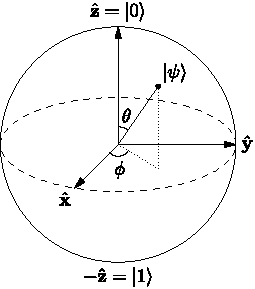
\includegraphics{images/chapter1/Bloch_Sphere.pdf}
    \caption{General rappresentation of a qubit state $|\psi\rangle$ on the Bloch sphere}
    \label{fig:BlochSphere}
\end{figure}

\noindent Each state coincides with each point present on the surface of the sphere, there is a one-to-one correspondence between a point on the surface and a state $|\psi\rangle$. We must underline the fact that the scalar product which we define in $\mathbb{C}^2$ is different from the scalar product in $S^2$, because, in the last one, $|0\rangle$ and $|1\rangle$ are in the same direction but opposite verse, so their scalar product is equal to -1 while in $\mathbb{C}^2$ is equal to 0. The Bloch sphere is a useful technique to visualize the qubit states.
\newpage

%%%%%%%%%%%%%
% LECTURE 2 %
%%%%%%%%%%%%%

\noindent \lecture{2}{08/10/2021}
\begin{itemize}
    \item \textbf{Postulate II}: What can we measure? In QM we measure observables and they are described from a self-adjoint operator:
    \begin{equation*}
        \hat A: \mathcal{H}\rightarrow \mathcal{H}
    \end{equation*}
    where $\hat A^\dagger=\hat A$, more specifically $\hat A^\dagger = (A^\intercal)^* \Rightarrow (A^\dagger)_{ij}=A^*_{ji}$
\end{itemize}
\noindent According to what we saw in the braket notation ($\bra{\phi}=\ket{\phi}^\dagger$), we will therefore have:
\begin{equation*}
    \ket{\psi}=B\ket{\phi} \Rightarrow \bra{\psi}=\bra{\phi}B^\dagger
\end{equation*}
\noindent Focusing on self-adjoint operators, we recall an important theorem of linear algebra:
\begin{theorem}[\textbf{Spectral Theorem}]
    Suppose $\hat A$ is a self-adjoint operator on a (real or complex) Hilbert space $\mathcal{H}$. Then there is an orthonormal basis of $\mathcal{H}$ consisting of eigenvectors of $\hat A$, which we denote as $\ket n$. Each eigenvalue $a_n$ is real.
    \begin{equation*}
        \hat A\ket n = a_n \ket n \text{ where } \ip{n}{m} = \delta_{ij}
    \end{equation*}
\end{theorem}
\noindent An important consequence to underline is that the number of orthonormal eigenvectors $\ket n$ is equal to the dimension of the Hilbert space that contains them, and being \textit{linearly independent} and \textit{orthonormal} (therefore orthogonal) they are a \textit{basis} for the Hilbert space under consideration. Being a basis, we can expand any state $\ket \psi$ as a linear combination of eigenvectors $\ket n$:
\begin{equation*}
    \ket \psi = \sum_{n=1}^N\alpha_n\ket n
\end{equation*}
\noindent where $\alpha_n\in\mathbb{C}$, $N=\text{dim } \mathcal{H}$.

\noindent Returning to our case of a two-level system, the Hilbert space we consider is $\mathbb{C}^2$ and we have taken the states $\ket 0 = \begin{pmatrix} 1 \\ 0 \end{pmatrix}$, $\ket 1 = \begin{pmatrix} 0 \\ 1 \end{pmatrix}$ as \textit{canonical basis} (also know as \textit{computational basis}). In this vector space, our operators are represented by a $2\times2$ matrices. In order to satisfy the self-adjoint condition, the matrix representation of a generic operator $\hat A$ must be expressed as:
\begin{equation*}
    \hat A = \begin{pmatrix}
        a+b & c-id \\ 
        c+id & a-b
    \end{pmatrix}
\end{equation*}
\noindent where $a, b, c, d \in \mathbb{R}$.
As we have decomposed a generic state vector $\ket \psi$ through a linear combination of eigenvectors $\ket n$, we can decompose a generic operator $\hat A$ as:

\begin{equation*}
    \hat A = a\mathbb{I}+b\sigma_1+c\sigma_2+d\sigma_3
\end{equation*}

\noindent where $\mathbb{I}$ is the \textbf{identity} and $\sigma_1, \sigma_2, \sigma_3$ are the \textbf{Pauli matrices}:

\begin{equation*}
    \mathbb{I}=
    \begin{pmatrix}
        1 & 0 \\
        0 & 1
    \end{pmatrix} \ \ \ \ \
    \sigma_1=
    \begin{pmatrix}
        0 & 1 \\
        1 & 0
    \end{pmatrix} \ \ \ \ \
    \sigma_2=
    \begin{pmatrix}
        0 & -i \\
        i & 0
    \end{pmatrix} \ \ \ \ \
    \sigma_3=
    \begin{pmatrix}
        1 & 0 \\
        0 & -1
    \end{pmatrix} \ \ \ \ \
\end{equation*}

\noindent They are used in the spin description as $\hat{\vec{S}}=\frac{\hbar}{2}\hat{\vec{\sigma}}$.\\
Now let's look at the eigenvalues and eigenvectors of Pauli matrices:
\begin{center}
    \begin{tabular}{clc}
        \hline
        \textbf{Pauli matrices} & \textbf{Eigenvectors} & \textbf{Eigenvalues} \\ \hline \\
        $\hat \sigma_1$ & $\ket + = \frac{1}{\sqrt 2}\begin{pmatrix} 1 \\ 1\end{pmatrix}, \ \ \ \ \ \ket- = \frac{1}{\sqrt 2}\begin{pmatrix} 1 \\ -1\end{pmatrix} $ & \{1,-1\}\\ \\
        $\hat \sigma_2$ & $\ket i = \frac{1}{\sqrt 2}\begin{pmatrix} 1 \\ i\end{pmatrix}, \ \ \ \ \ \ket{-i} = \frac{1}{\sqrt 2}\begin{pmatrix} 1 \\ -i\end{pmatrix} $ & \{1,-1\}\\ \\
        $\hat \sigma_3$ & $\ket 0 = \begin{pmatrix} 1 \\ 0\end{pmatrix}, \ \ \ \ \ \ket 1 = \begin{pmatrix} 0 \\ 1\end{pmatrix} $ & \{1,-1\} \\ \\ \hline
    \end{tabular}
\end{center}

\noindent We observe, for example, that
\begin{equation*}
    \ket + = \frac{\ket 0 + \ket 1}{\sqrt 2} \ \ \ \ \ \ket - = \frac{\ket 0 - \ket 1}{\sqrt 2}
\end{equation*}
\noindent We can see these new bases on the Bloch sphere.
\newline
\begin{figure}[!ht]
    \centering
    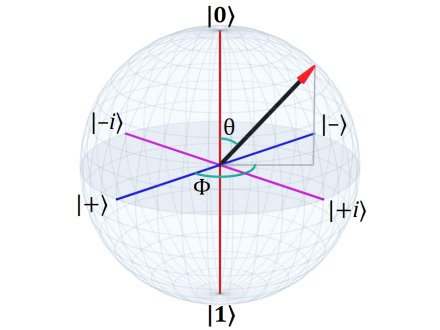
\includegraphics[scale=0.5]{images/chapter1/bloch-hdr-440.png}
    \label{fig:BlochSphere2}
\end{figure}
\newline
\noindent If we define the spin along a generic direction $\vec n = (\cos\phi\sin\theta, \sin\phi\sin\theta, \cos\theta)$, then along $\vec n$ we will have:
\begin{equation*}
    \hat{\vec{\sigma}} \cdot \vec n = \cos\phi\sin\theta\sigma_1+\sin\phi\sin\theta\sigma_2+\cos\theta_3
\end{equation*}
\begin{itemize}
    \item \textbf{Postulate III}:
    \begin{enumerate}
        \item \textbf{Measurement}: Let's take the operator self-adjoint $\hat A$, with his base $\ket n$ where we have $\hat A\ket n=a_n\ket n$, and $a_i\neq a_j \ \forall i\neq j$. We can expand $\ket \psi$ on $\ket n$ base, such that $\ket \psi = \sum_n \alpha_n\ket n$. By measuring the quantity $A$, we obtain the value $a_n$ with probability equals to $|\alpha_n|^2$. (We already assumed that $|\psi|^2=1$).
        \item \textbf{Collapse of the wave function}: After the measure what happens to the $\psi$ state? When we do a measure, instantly $\ket \psi$ collapse to the state $\ket n$ which gave us the $a_n$ value: $\ket \psi \rightarrow \ket n$. If we do another measure on $\ket \psi$, we get again $\ket n$ with a probability of $1$ (\textbf{Born's rule}).
    \end{enumerate}
\end{itemize}
\noindent Let's consider for a qubit $\ket \psi$ ($\text{dim} = 2$) the most general state:
\begin{equation*}
    \ket \psi = \cos \frac{\theta}{2}\ket 0+\sin \frac{\theta}{2}e^{i\phi}\ket 1
\end{equation*}
\noindent If we perform an experiment to measure a spin, in the z-basis ($\sigma_3: \{\ket 0, \ket 1\}$) the probabilities will be:
\begin{equation*}
    P(\ket 0) = \bigg|\cos^2\frac{\theta}{2}\bigg| \ \ \ \ \ P(\ket 1) = \bigg|\sin^2\frac{\theta}{2}\bigg|
\end{equation*}
\noindent we must note that: $P(\ket 0)+P(\ket 1)=1$\\
Instead, if we consider the x-basis ($\sigma_1: \{\ket +, \ket -\}$) our $\ket \psi$ state will be:
\begin{equation*}
    \ket \psi = \frac{1}{\sqrt 2}\bigg(\cos\frac{\theta}{2}+e^{i\phi}\sin\frac{\theta}{2}\bigg)\ket + + \frac{1}{\sqrt 2}\bigg(\cos\frac{\theta}{2}-e^{i\phi}\sin\frac{\theta}{2}\bigg)\ket -
\end{equation*}
\noindent the new probabilities will be:
\begin{equation*}
    P(\ket +)=\frac 12 \bigg|\cos\frac{\theta}{2}+e^{i\phi}\sin\frac{\theta}{2}\bigg|^2
\end{equation*}
\begin{equation*}
    P(\ket -)=\frac 12 \bigg|\cos\frac{\theta}{2}-e^{i\phi}\sin\frac{\theta}{2}\bigg|^2
\end{equation*}
\noindent Let us now analyze the following situation, suppose we have a psi state written as a linear combination of $\ket+$ and $\ket-$. If during the measurement of the x-component of $\ket \psi$ we obtain $\ket+$, a subsequent measurement, always of the same component, will produce the same result with a probability of $100\%$. Now we know that we are in the $\ket+$ state, let's measure the component along x. By the Heisenberg uncertainty principle we will have:
\begin{equation*}
    P(\ket+)=\frac 12 \ \ \ \ \ P(\ket-)=\frac 12
\end{equation*}
\noindent The same goes for all directions as: 
\begin{equation*}
    [\hat S_i, \hat S_j]=i\hbar\varepsilon_{ijk}\hat S_k
\end{equation*}
\noindent Suppose we have \textbf{degeneration} on $\ket\psi$, this means that some eigenvalues are equal to each other, associated with different eigenstates: 
\begin{equation*}
    \ket \psi = \alpha_1\ket1+\alpha_2\ket2+\alpha_3\ket3+\alpha_4\ket4+\alpha_5\ket5\alpha_6\ket6
\end{equation*}
\noindent where we suppose the degeneracy on $a_1=a_2$ and $a_4=a_5=a_6$. 
\begin{equation*}
    \ket \psi = \underbrace{\alpha_1\ket1+\alpha_2\ket2}_{\hat P_{a_1}\ket\psi}+\underbrace{\alpha_3\ket3}_{\hat P_{a_3}\ket\psi}+\underbrace{\alpha_4\ket4+\alpha_5\ket5\alpha_6\ket6}_{\hat P_{a_4\ket \psi}}
\end{equation*}
\noindent To describe this situation we introduce \textbf{projectors} $\hat P_{ai}$ with their following properties:
\begin{enumerate}
    \item $\hat P_a^\dagger=\hat P_a$
    \item $\hat P_a^2=\hat P_a$
    \item $\sum_i \hat P_{a_i}=\mathbb{I}$
\end{enumerate}
\noindent These are useful for treating Born rule, in the previous case we have 3 possible outcomes. And the probability to get these outcomes is:
\begin{equation*}
    P(a_n)=||P_{a_n}\ket \psi||^2
\end{equation*}
\noindent After the measurement, our wave function will collapse to the normalized state:
\begin{equation*}
    \ket \psi \rightarrow \frac{P_{a_n}\ket\psi}{||P_{a_n}\ket \psi||}
\end{equation*}
\noindent For example, if we look at the probability of getting $a_1=a_2$, we'll get:
\begin{equation*}
    P(a_1)=||\alpha_1\ket1+\alpha_2\ket2||^2=|\alpha_1|^2+|\alpha_2|^2 \ \ \ \text{Parseval Identity}
\end{equation*}
\noindent What happens to the state $\ket \psi$? It will collapse in the state (properly normalized):
\begin{equation*}
    \ket \psi=\frac{1}{\sqrt{|\alpha_1|^2+|\alpha_2|^2}}\big(\alpha_1\ket1+\alpha_2\ket2\big)
\end{equation*}
\noindent Now I have an uncertainty about $\ket\psi$ for $\ket1$ or $\ket2$, but if I can realize an experiment that allows me to solve the degeneration, I will have a well-defined state (think about H atom).
\begin{itemize}
    \item \textbf{Postulate IV}: The last postulate states that time evolution is described by the Schrödinger equation:
    \begin{equation*}
        i\hbar\frac{d}{dt}\ket{\psi(t)}=\hat H \ket{\psi(t)}
    \end{equation*}
    where $\hat H$ is the hamiltonian operator and it is self-adjoint.
\end{itemize}
\noindent An important thing to note is the fact that the probability is conserved:
\begin{equation*}
    \ip{\psi(t)}{\psi(t)}=\ip{\psi(0)}{\psi(0)}=1
\end{equation*}
\noindent When we solve Schrödinger equation, we get, by introducing the so call \textbf{time operator} $\hat U(t)$:
\begin{equation*}
    \ket{\psi(t)}=\hat U(t)\ket{\psi(0)}
\end{equation*}
\noindent if $\hat H$ is time-indipendent:
\begin{equation*}
    \hat U(t) = e^{-\frac{i}{\hbar}\hat H t}
\end{equation*}
\noindent if $\hat H = \hat H(t)$, we have to distinguish the case of commutating and non-commutating hamiltonians at different times.\\
The fact that in time evolution, the probability is preserved, is due to the fact that $\hat U(t)$ is a unitary operator:
\begin{itemize}
    \item $\hat U \hat U^\dagger=\hat U^\dagger U = \mathbb{I}$
    \item $\ip{\hat U\phi}{\hat U\psi}=\ip{\phi}{\hat U^\dagger \hat U\psi}=\ip{\phi}{\mathbb{I}\psi}=\ip{\phi}{\psi}$
\end{itemize}
\noindent Since it is a unitary operator:
\begin{equation*}
    \hat U^\dagger\hat U = \bigg(e^{-\frac i\hbar \hat H t}\bigg)^\dagger e^{-\frac i\hbar \hat H t} = e^{\frac i\hbar \hat H t} e^{-\frac i\hbar \hat H t} = \mathbb{I}
\end{equation*}

\section{Gates}

\begin{definition}[\textbf{Quantum Circuit}]
    A \textbf{quantum circuit} is a model of quantum computing where there is an ordered sequence of \textbf{quantum gates} that are applied to the \textbf{qubits}.
\end{definition}

\begin{definition}[\textbf{Quantum Gates}]
    The quantum analogue of the classical logic gates are the \textbf{quantum gates}. The main difference from the classic case lies in the fact that we cannot directly implement all the ports classics like and, or, xor, \dots
\end{definition}
\noindent If in classical circuits, the use of logic gates is trivial, think of the \texttt{NOT} gate:
\newline
\begin{center}
    \begin{circuitikz}
        \draw
        (0,4.5) node[not port] (mynot) {}
        (mynot.in) node[left =.4cm, anchor=east] (a) {$0$}
        (mynot.out) node[right = .4cm,anchor=west] (b) {$1$}
        (mynot.in) -- (a)
        (mynot.out) -- (b)
        (0,3) node[not port] (mynot) {}
        (mynot.in) node[left =.4cm, anchor=east] (a) {$1$}
        (mynot.out) node[right = .4cm,anchor=west] (b) {$0$}
        (mynot.in) -- (a)
        (mynot.out) -- (b);
    \end{circuitikz}
\end{center}
\noindent In a \textbf{qubit} we can do more things and these will be described from an hamiltonian:
\begin{center}
    \mbox{
        \Qcircuit @C=1em @R=1em {
            \lstick{\ket{\psi}} & \gate{\hat U} & \rstick{\hat U\ket{\psi}} \qw \\
        }
    }
\end{center}
$\hat U$ can be any unitary operator like $\hat U = e^{-\frac{i}{\hbar}\hat H t}$ where $\hat H$ describes a given phenomena. Since \textbf{Pauli matrices} are unitary: $\sigma_i^\dagger=\sigma_i$, $\sigma_i^2=\mathbb{I}$, if we want to study, for example, the spin of a particle inside a magnetic field, then: $\hat H = \vec \sigma \cdot \vec B$.
